\chapter{Introduction} \label{chap_introduction}

\section{Background} \label{sec_background} 

There is this notion that everything is always in motion, a constant state of flux. This
notion has been recognized for centuries and is famously described by the Greek
philosopher
\emph{Heraclitus}\footnote{\url{https://plato.stanford.edu/entries/process-philosophy/}}
with his statement \emph{Pantha Rhei} (Everything flows). This notion is particularly
relevant in the context of software engineering, as software systems must be able to
evolve and adapt to changing business requirements.

Software engineering is constantly evolving as new technologies, methodologies, and best
practices are developed to meet the demands of modern corporate environments. In this
context, the concept of software stability is a constant reality. Software systems must be
able to evolve and adapt to changing business requirements over time. However, this
evolution must be managed to maintain the stability of software artifacts.

The laws of software evolution describe the balance between the forces driving new
requirements and those that slow down progress. As a result, changing software can lead to
deterioration in stability and evolvability, which can negatively impact the quality of
these systems. Scholars have recognized this challenge for decades, and much research has
conducted to address it \parencite{lehman_programs_1980}.

\section{Related work} \label{sub:related_work}

Early pioneers in software engineering recognized the importance of modular programming
practices to improve code clarity and maintainability. James Edwin McIlroy proposed a
vision where the systematic reuse of software building blocks leads to more abstraction of
repetitive tasks, and eventually reduces the complexity \parencite[79]{p_naur_nato_1968}. 

Dijkstra argued against using unstructured control flow in programming and advocated for
using structured programming constructs to improve the clarity and maintainability of code
\parencite{dijkstra_letters_1968}. He advocated structured programming techniques that
improved the modularity and evolvability of software artifacts. Parnas continued with the
principle of information hiding. He stated that design decisions used multiple
times by a software artifact should be modularized to reduce complexity
\parencite{parnas_criteria_1972}. 

Various programming paradigms, including procedural, object-oriented, and functional
programming, have emerged to enhance software programming capabilities. In addition, these
paradigms have impacted modern programming languages, such as Java and C\#, enabling the
development of more modular and evolvable software architectures.

\section{Research Problem: The plethora of proposed design \\ principles}
\label{sec_research_problem}

Design principles, patterns, and theorems are, on top of all, additional measures to
enhance the modularity, stability, and evolvability of software artifacts. This thesis
focuses on two prevalent approaches to researching the hypothesized convergence, namely
\gls{ns} and \gls{ca}. introduced in \ref{sec_into_ca} and \ref{sec_inro_ns}. 

A wide variety of proposed design principles are available for the challenges that occur
in modular and evolvable software architecture. Many great experiences documented
throughout professional and personal blog posts on the internet \parencites{noauthor_dont_nodate,
noauthor_generalization_nodate, noauthor_law_nodate}. Unfortunately, many
experiences have mixed outcomes, some are opinionated, and results are sometimes based on
improper interpretations of the proposed solutions.

Deciding on the best fit for one of the solutions is a recurring and often challenging task
for software architects. A popular and widely accepted solution from software engineering
literature is \gls{ca}. There is a broad supporting community, and many corporate
solutions move toward architectures similar to the \gls{ca}
approach. 

An architecture that derives from science and empirical evidence is \gls{ns}
\parencite{mannaert_normalized_2009,mannaert_normalized_2016}. Deciding between the two
approaches can be a challenging task with little documentation and research. Is it
possible that combining the two approaches can be an method that leads to a highly modular
and evolvable software artifact? Let us start with a small introduction to both
approaches.
\section{Introduction to Clean Architecture} \label{sec_into_ca}

\ca is the accumulation of more than half a century of coding, designing, and
architecting software systems by \citeauthor*[]{robert_c_martin_clean_2018}. He published
his experience in his book \citetitle*[]{robert_c_martin_clean_2018} in
\citeyear[]{robert_c_martin_clean_2018}. In this book, he states that creating a software
artifact requires less skill and knowledge. However, creating stable and evolvable
software artifacts is a skill that requires a lot of knowledge, skill, dedication, and
time.

The book aims for a software architecture that minimizes the human resources required to
build and maintain the information system. Like \ns, it has a
prescribed design of software classes that will lead to a modular architecture with low
coupling and high cohesion \parencite{robert_c_martin_clean_2018}.

\section{Introduction on Normalized Systems} \label{sec:inro_ns}

The Normalized Systems theorems are a scientific approach to creating software systems
based on the laws for software evolvability. These theorems have resulted in a documented
track record of achieving software stability, in a scientific environment. Effectively, it
prevents the accumulation of combinatorial effects on anticipated change drivers. This
prevents the positive feedback loop and prevents the degradation of the software artifact.
Preventing positive feedback loops has a positive effect on the evolvability of software
artifacts.\parencite[]{mannaert_normalized_2009}. 

\citeauthor[]{mannaert_normalized_2009} have formulated the theorem of Normalized Systems
as prescriptive structures (elements) that lead to a modular architecture with low
coupling and high cohesion. The resulting software architecture will be designed to cope
with future change \parencites[]{mannaert_normalized_2009}.
\section{Hypothesis} \label{hypothesis} 

The proposed hypothesis is that both 'Clean Architecture' and 'Normalized Systems' lead
to a modular software architecture with reduced combinatorial effects. Consequently, both
architectural approaches will lead to improved stability and evolvability of the
Information system.

Both architectural approaches formulate their modular structures independent of any
given programming technology \parencite[]{mannaert_normalized_2009,martin_clean_2018}. As
such, improvements in terms of stability and evolvability are equally applicable for the
C\# artifact used in this research, compared to case studies where Java SE has been used.
\parencites[]{oorts_building_2014, de_bruyn_enabling_2018}.

\begin{figure}[!ht]
    \centering
    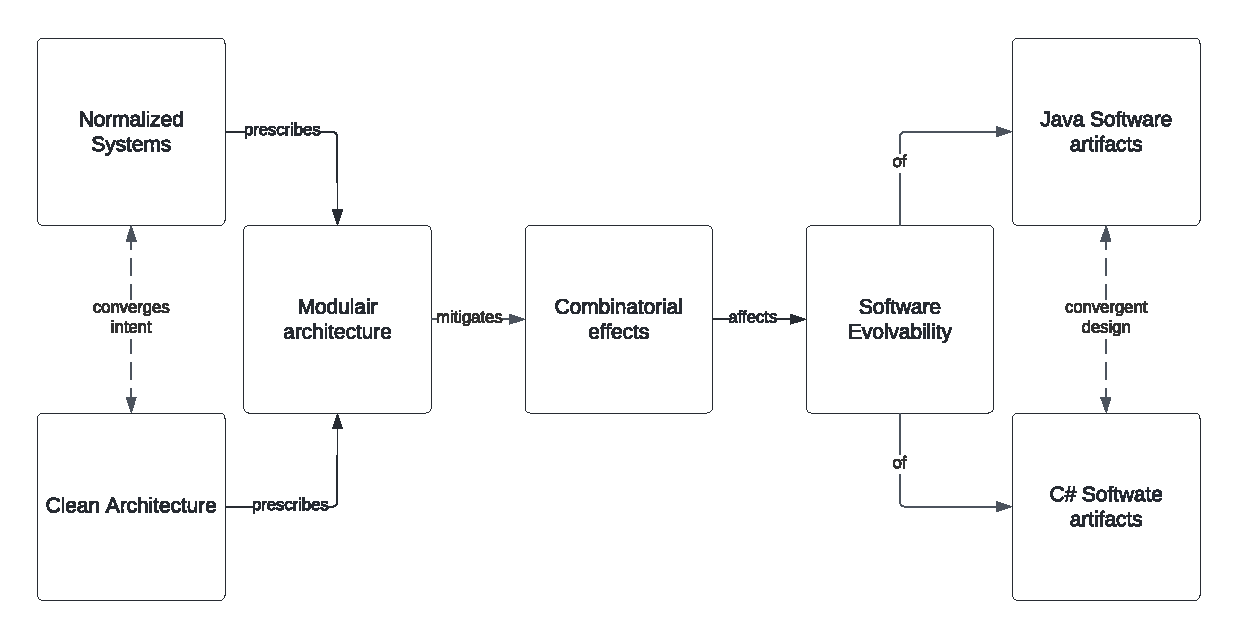
\includegraphics[width=0.9\textwidth]{Figures/hypothesis.pdf}
    \caption[The hypothesis]{The hypothesis}
    \label{fig_hypothesis}
\end{figure}
\section{Research Objectives} \label{sec_research_objectives}

In this Design Science Research, we will shift the focus from Research Questions to
Research Objects. The Object of this research is to determine the degree of convergence of
Clean Architecture, with the Normalized Systems Theory. 

To summarize, we will start with a generic design that is based on the principles and
design characteristics of Clean Architecture. Given this design, we will conduct the
research on two different artifacts, namely a code-generator artifact and a generated
artifact. The reason for the code-generator artifact is to provide strict and meticulous
adherence to the generic design. Each entity should be implemented in exactly the same way.

AFMAKEN



% In this Design Science research, the focus shifts from a research question toward
% research objectives. The following objectives apply to this research.

% \subsection*{Objective 1: The expander artifact}
% A C\# artifact that consists of a source code expander and some helper classes to
% generate the second \emph{expanded} artifact. The artifact supports the harvesting and
% rejuvenation of custom code snippets on the expanded artifact so that regenerations do not
% have a loss of implementations on the expanded artifact. The expander artifact is entirely
% based on the design principles of \gls{ca}.

% Chapter \ref{sec_generator_artifact} entirely describes the expander artifact.

% \subsection*{Objective 2: The expanded artifact}
% This artifact is an entirely working restful API, that is based on ASP.NET and C\#. It has
% essential CRUD support. The artifact has been generated by the \emph{expander} and has
% been enriched with custom code snippets to comply with the initial requirements.
% The expanded artifact is entirely based on the design principles of \gls{ca}.

% Chapter \ref{sec_generator_artifact} entirely describes the expander artifact.


\section{Research questions} \label{research_questions}
The Hypothesis described in \ref{hypothesis} and \ref{conceptualframework} leads us to the
following research question:

\begin{center}
    \enquote*{\textit{To what extent converges the evolvability of a C\# artifact built
    based on the Clean Architecture principles towards a similar artifact that is based on
    Normalized Systems Theorems?}}
\end{center}

The following sub-questions can be formulated that support the research on the main
research question:
\begin{itemize}
    \item How does Clean Architecture contribute to Software Evolvability?
    \item To what extent Is Normalized Systems applicable to a C\# artifact?   
\end{itemize}
\section{Research method} \label{sec_research_method}

This research is a Design Science Method and relies on the Engineering Cycles as described
by \textcite{wieringa_design_2014}. The engineering cycle provides a structured approach
to develop the required artifacts to analyze the design problem (HIER CITE NAAR WIERINGA).

\begin{figure}[H]
    \centering
    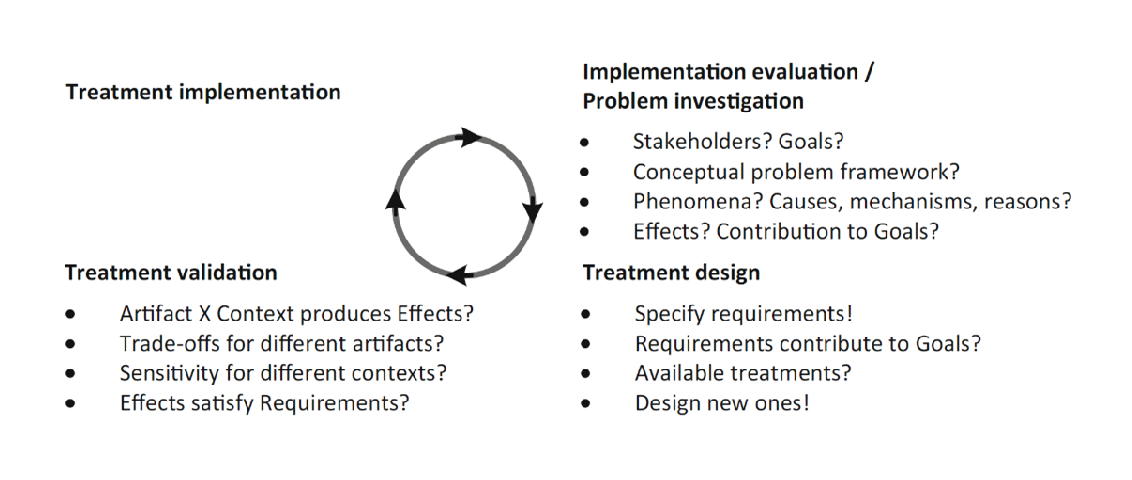
\includegraphics[width=1\textwidth]{Figures/engineering_cycle.pdf}
    \caption[Engineering cycle]{Wieringa's engineering cycle}
    \label{fig_engineering_cycle}
\end{figure}

In the context of this research, the artifacts described in chapters
\ref{sec_generator_artifact} and \ref{sec_generated_artifact} are considered to be
information systems. \citeauthor{hevner_design_nodate} proposed a framework for research
in information systems by introducing the interacting relevance and rigor cycles.

Figure \ref{fig_dsr} depicts a specialized overview of Hevners Design Science Framework.
The rigor cycle is composed of the theories and knowledge from \gls{ns}
and \gls{ca}. This is supplemented by the rigorous knowledge of modularity,
evolvability, and stability of software systems. The Relevance cycle represents the
business needs of the stakeholders. The business needs are described as research
objectives, research questions, and research requirements.

\begin{figure}[H]
    \centering
    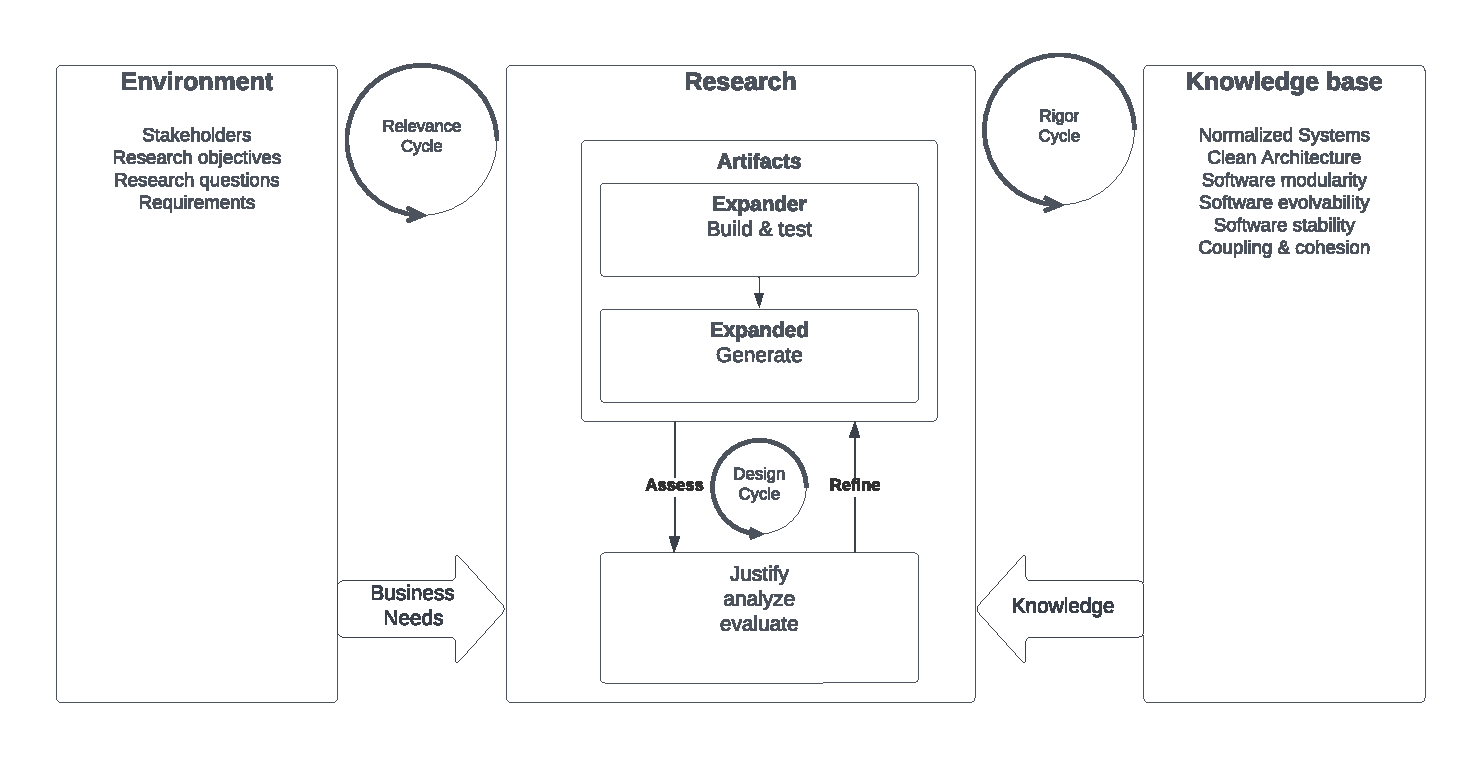
\includegraphics[width=1\textwidth]{Figures/rigor_relevance_cycle.pdf}
    \caption[DSF]{The Design Science Framework for IS Research}
    \label{fig_dsr}
\end{figure}
\section{Thesis outline} \label{sec_structure}

The structure of this thesis reflects the research methodology described in the previous
section \ref{sec_research_method}. Chapter \ref{chap_theoreticalbackground} presents the
theoretical backgrounds of both \ns and \ca, discussing important
characteristics and requirements of software stability, as well as the principles and
architectures proposed by both development approaches.

Chapter \ref{chap_requirements} focuses on the requirements relevant to this research. It
is divided into two sections: section \ref{sec_research_requirements} outlines the
research requirements, describing the requirements necessary for conducting the research,
while section \ref{sec_artifact_requirements} details the artifact requirements, laying
out the requirements relevant to the artifacts contributing to this research.

Chapter \ref{chap_evaluation} evaluates the research results, discussing the impact of
using CA on NS. Notable experiences and findings in Chapter \fullref{chap_discussion}. The
conclusion of this research is presented in the final chapter, Chapter \ref{chap_conclusions}.

Lastly, it is worth mentioning that this thesis follows the guidelines of the American
Psychological Association (APA) style, including the use of US spelling.